\chapter{Dimensional Dependence of Optical Transition Rates} \label{RM}
 
\section{Time-dependent Perturbation Theory} \label{dust_seds}

\subsection{} \label{dust_corrections}

%\subsection{A Uniform Sample}
%\subsection{\ltwofive\ and \bctwofive\ Distributions} \label{l_bc_dust}
%\subsection{Extinction Corrected SEDs} \label{l_bc_dust}

\section{Upward and Downward Transition Rates} \label{mbh_seds}

\section{Contributing Factors} \label{BH_conclusions}
\subsection{Overlap Integral}
\subsection{Oscillator Strength}
\subsection{Joint Optical Density of States}

The preceding theory of gain involving Fermi's Golden Rule considers each
electron in isolation as it interacts with the electromagnetic field. In other
words, we have used a single-particle theory to obtain the gain spectrum. In
reality, there is a large density of both electrons and holes present in the
system. The mutual interactions between these particles are generally referred
to as many-body effects. These effects included lineshape broadening, which is
related to collisions between particles and/or phonons in the crystal. In
addition to this important effect, there are two other significant consequences
of many-body effects: exciton states and bandgap shrinkage. Exciton states
exsit primarily at low carrier densityies and low temperatures, where bandgap
shrinkage becomes noticeable at high carrier densities.

Under conditions of low carrier density and low temperature, it is possible for
an electron and hole to orbit each othere for an extended period of time,
forming what is referred to as an exciton pair. Such exciton pairs have a
binding energy associated with them that is euqal to the energy required to
separate the electron and hole. As a rsult, electrons that are elevated from
the valence band to one of these exciton states will absorb radiation at
energies equal to the bandgap less the binding energy (the bandgap will appear
to be red-shifted). More significatnly however, the overlap integral ( and
hence the matrix element ) of these two-particle states can be quite large. As
a result, band-to-exciton transitions tend to dominate the absorption spectrum.
However, exciton states are limited to states near $k = 0$, and hence
band-to-exciton transitions are clustered at the band edge (or subbabdn edge).
The overall effect is the qppearance of very strong absorption peaks near the
subband edges in quantum-well materials, and near the band edge in bulk
material.

Exciton absorption peaks are clearly visible in quantum wells at room
temperature for a typical GaAs QW. The first two steps in the "staircase"
absorption spectrum predicted from the density of states. However, the exciton
peaks riding on top of the steps, particularly the n = 1 peaks, dominate the
absorption spectrum. Each observed exciton peak corresponds to one of the
subband transitions.

The second many-body effect occurs at high carrier densities, where the charges
actually screen out the atomic attactive forces. With a weaker effective atomic
potential, the single-atom electron wavefunctions of interest become less
localized and the nearest-neighbor electron everlap becomes higher.  The large
overlap increases the width of the energy bands ($\delta{E}$ is larger),
reducing the gap between bands. Although this description is only qualitative,
it does reveal that the bandgap should shrink with increasing carrier density.

It can also be argued theoretically that the badgap shrinkage is inversely
related to the average spacing between carriers, or (the closer the carriers
are, the more their own Coulomb potentials screen out the atomic potential). In
bulk material, the average volume occupied by one carrier is inversely related
to the carrier density. 

The net effect of bandgap shrinkage is that as carrier density increases, the
entire gain spectrum redshifts by a noticeable amount. In principle, the shift
is accompanied by a slight distortion. (i.e, reshaping and enhancement) of the
spectrum.

With decreasing dimensionality of the active region of an injection laser, the
density of states and gain spectra become narrower, which leads to a decrease
in the number of states to be filled to make the active region transparent
(zero population inversion and zero gain) and to achive lasing (gain equal to
loss) Consequently, the transparency current (or inversion current) at which
the gain is equal to the loss and lasing begins decrease and their temperature
dependences become weaker~\cite{asryan2004theory}.

Figure 8 (C) shows the FDTD-simulated electric field density of a hexagonal
nanowire at y cross section (top) and x cross section (bottom). The photon
energy of this mode shown as the insets of Fig. 8(C) is concentrated primarily
along the 6 corners and secondarily along the facets with little light in the
3D core of GaAs. Hence, we suggest that the fortuitous spatial overlap of the
resonant optical modes on reduced dimensional electronic wavefunctions plays a
significant role in the remarkable optoelectronic properties of core-shell
nanowires. Restated, the superposition of the photon modes  on reduced
electronic states that form on the facets and vortices of the hexagonal CSNWs
strongly enhances both upward and downward transition rates.  Thus, the reduced
dimensionality transition rate distinguishes the core-shell nanostructure from
the optically equivalent structures of Fig. 6 due to its significantly modified
rate management. These nanostructures are not only excellent optical cavities,
but despite their large size also provide the right reduced dimensional
electronic structures which enhance optoelectronic interactions.  It should be
noted the present analysis is for direct optical transitions; although it can
be extended to incorporate k-vector changes as in phonon scattering, other
important factors such as many-body interactions need to be included in a


\begin{figure}
  \caption{Photon Charge Distribution}
  \centering
  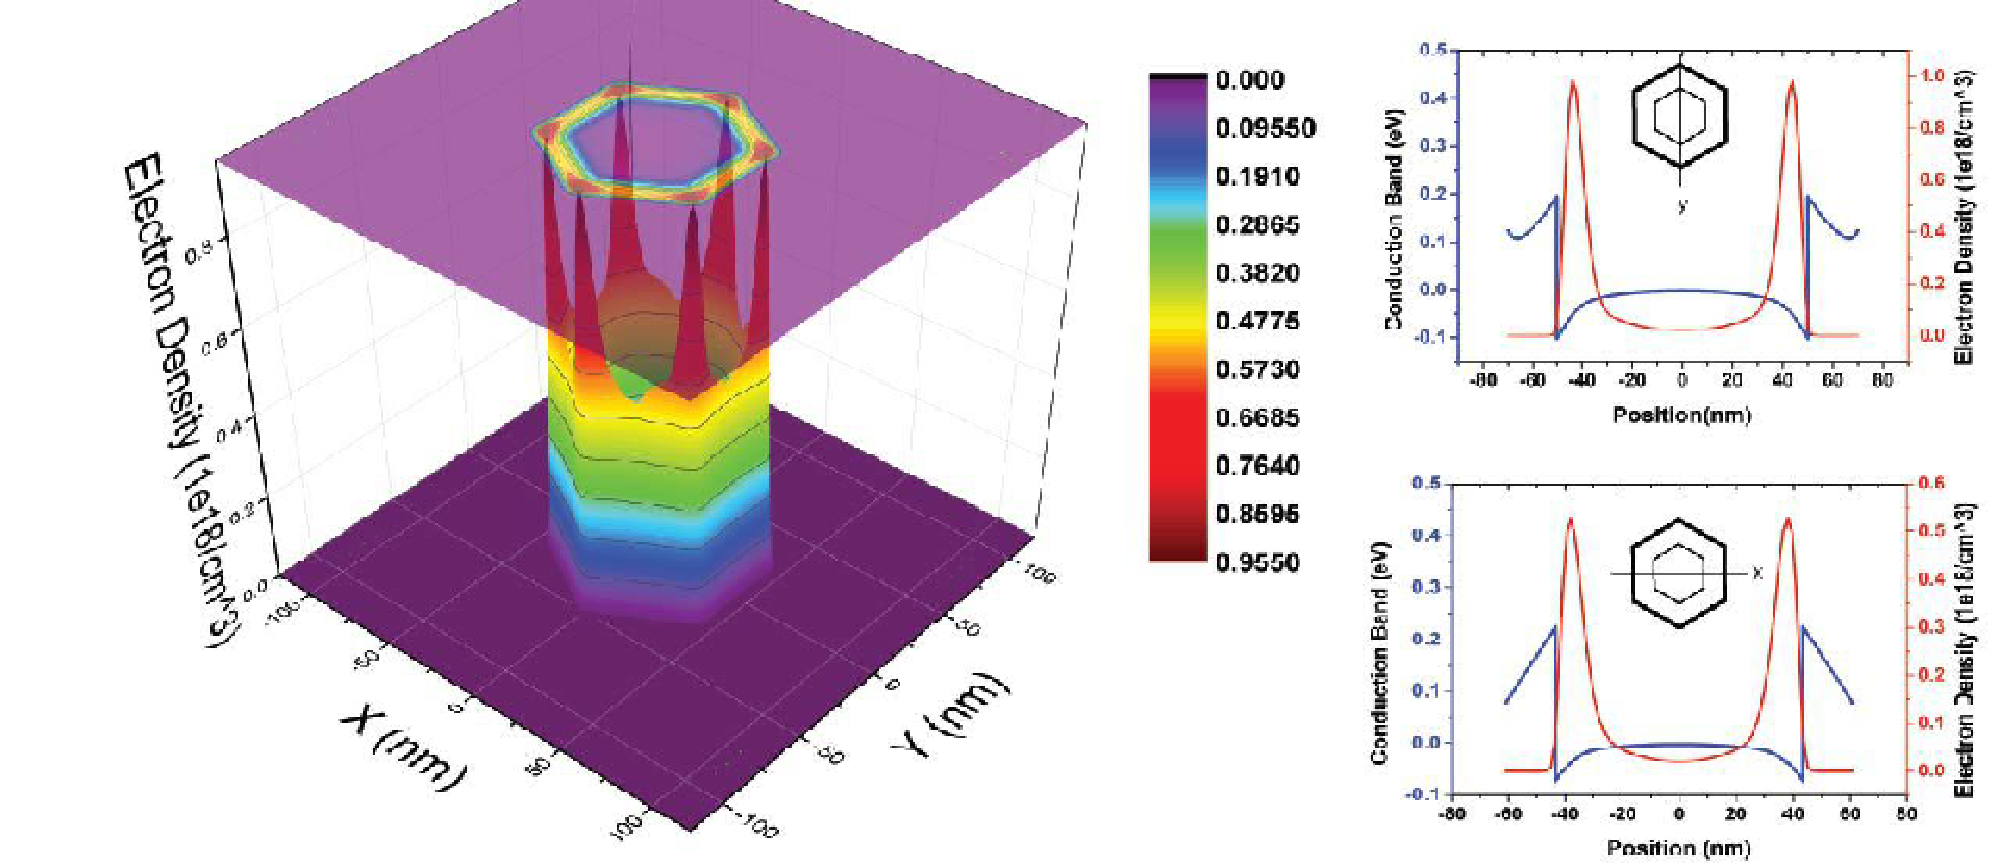
\includegraphics[width=\textwidth]{pictures/ED/Photoncharge}
  \label{PhotonCharge}
\end{figure}


